\chapter{Realizace zařízení}
Tato kapitola popisuje kompletní návrh řešení rozšíření komernčně používaného sytému o senzorovou síť.

%%%%%%%%%%%%%%%%%%%%%%%%%%%%%%%%%%%%%%%%%%%%%%%%%%%%%%%%%%%%%%%%%%%%%%%%%%%%%%%%%%%%%%%
\section{Implementace WSN do přístupového systému}
\label{Implementace WSN do přístupového systému}
Přístupový systém k rozšíření o WSN pro tento projekt je vytvořen firmou IMA a je komernčně distribuován. Jeho architektura se liší od všeobecné architektury zobrazené v blokovém schematu \ref{fig:Access control system architecture} přidáním zařízení CKP, tvořícího rozhranní mezi kontrolním panelem a čtečkou s dveřním zámkem. Přístupový systém má několik typů CKP zařízení podporujících různé typy čteček, dveřních zámků, závor, vrat apodobně, ale všechna tato CKP zařízení podporují CKP protokol v síti RS485 pro komunikaci s kontrolním panelem.

Rozšíření tohoto Přístupového systému o WSN je vytvořeno připojením WSN gatewaye ke kontrolnímu panelu přes RS485 síť stejně jako CKP zařízení. Názorná blokové schéma přístupového systému firmy IMA s implementací WSN gatewaye je zobrazeno v obrázku \ref{fig:ACS architecture IMA with geteway}.
V budovách, kde již je tento přístupový systém nainstalován je obvykle více kontrolních panelů, vždy jeden kontrolní panel pro několik dveří s CKP zařízeními propojenými sítí RS485. 
K jednomu přístupovému systému je možné přípojit několik WSN gatewayí k libovolným kontrolním panelům v budově pro dosažení požadovaného pokrytí WSN.

\begin{figure}[!h]
\centering
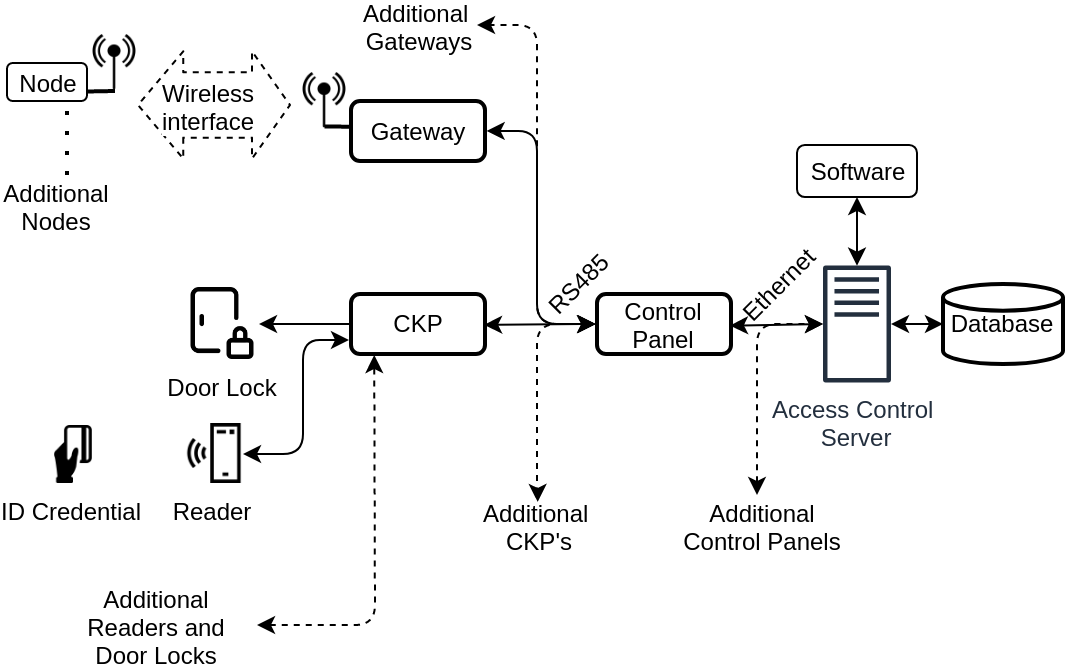
\includegraphics[width=1\textwidth]{ACS_IoT_extension_21}
\caption{IMA access control system architecture with WSN extension}
\label{fig:ACS architecture IMA with geteway}
\end{figure}


WSN gateway tedy musí podporovat CKP protokol v sítí RS485 navržen firmou IMA. Jedná se o kolizní protokol, kde všechna zařízení se řídí pravidlem "listen before talk", kolize jsou detekovány 
mechanismem kontroly integrity použitý v každé zprávě. V případě že zařízení přijme poškozený příkaz, vyžádá jeho opakování.

Přístupový systém firmy IMA funguje tak, že CKP zařízení získává seznam všech platných karet (ID Credentials) ze serveru řízení přístupu a na základě tohoto seznamu pak CKP zařízení provádí odpovídající akci po přiložení karty ke čtečce. 
Je-li ke čtečce přiložena karta, jejíž číslo není obsaženo v seznamu platných karet, CKP zařízení pouze signalizuje událost uživateli (např. červené bliknutí nebo pípnutí), ale zprávu o této události neodesílá na server řízení přístupu. Je-li ke čtečce přiložena karta, jejíž číslo je obsaženo v seznamu platných karet, CKP zařízení signalizuje událost uživateli (např. zelené bliknutí nebo pípnutí) a zprávu o této události odesílá na server řízení přistupu příkazem tzv. "průchod".
Navržená gateway bere seznam platných karet jako seznam platných koncových zařízení senzorové sítě. Gateway pak zpracovává packety pouze od zařízení z tohoto seznamu a ostatní ignoruje, tudíž v síti RS485 jsou přenášena pouze relevantní data.
Data z koncových zařízení jsou odesílána na server řízení přístupu příkazem "průchod", který má fixní velikost a po přidání adresy koncového zařízení o velikosti 4 B zde už zbývá poze 6 B pro data z koncového zařízení, což je velké omezení.
%Since the CKP protocol allows to transmit fixed-size command with only 10 bytes of space, the first 4 bytes are LoRaWAN device address of the node from which the packet was received and the 6 remaining bytes are used for the node data.
LoRaWAN protokol používá packet, jehož samotná hlavička je o minimální velikosti 13 B. 
Různá LoRaWAN koncová zařízení používají různé velikosti payloadu, takže není možné odesílat celý payload koncového zařízení přes síť RS485.
Tento problěm je řešen ta, že LoRaWAN packety z koncových zařízení jsou dešifrovány přímo v gatewayi a konečné hodnoty senzorů jsou vypočítány z payloadu zařízení na základě dokumentace poskytnuté výrobcem \cite{RHF1S001 pdf}. Vybrané hodnoty jsou odeslány na server řízení přístupu skrze kontrolní panel. 
% In summary, when the Gateway receives an encrypted LoRaWAN packet, it looks for whether the Node device address is in the list of known device addresses.
% If this is the case, the packet is encoded in the communication protocol of the Gateway and sent to the Control Panel. If there is not enough space in communication protocol of the Gateway, the packet is decrypted and relevant data, i.e., sensor values, are selected.

% When the user presents his card to the Reader and the card ID matches one of the valid cards, the CKP device sends the data to the Access Control Server.
% The same procedure applies to the Gateway.
% When the Gateway receives data from a Node and the Node address matches one of the valid device address list, the Gateway sends the data to the Access Control Server.

%%%%%%%%%%%%%%%%%%%%%%%%%%%%%%%%%%%%%%%%%%%%%%%%%%%%%%%%%%%%%%%%%%%%%%%%%%
\section{Návrh WSN gatewaye}
Jak již bylo zmíňeno v předchozí sekci, gateway dešifruje packety z koncových zařízení a na základě typu koncového zařízení vypočítává z payloadu hodnoty senzorů z nichž vybrané odesílá na server řízení přístupu přes kontolní panel a to z důvodu datového omezení protokolu v síti RS485, do které je gateway připojena.
Pro každý podporovaný typ koncového zařízení musí být implementováno zpracování payloadu ve FW gatewaye. Pozdější přidání typů koncových zařízení tedy vyžaduje update FW gatewaye.
Gateway tedy má uloženou informaci o typu koncového zařízení společně s jeho LoRaWAN device address.

LoRaWAN protokol je zabezpečen šifrováním AES-128 na dva způsoby, a to zabezpečení aplikační pro nečitelnst přenášených dat a síťové pro zabránění pro zabránění útočníkům opakovat již přenesené packety nebo odesílat falešné packety. Jsou zde tedy dva AES-128 šifrovací klíče, applikační klič AppSKey (Application Session Key) a síťový klíč NwKSKey (Network Session Key).

Jelikož adresy koncových zařízení jsou předávány gatewayi stejně jako platné karty čtečce z aplikace na serveru řízení přistupu, není zde možnost předávávat dva 16 B dlouhé šifrovací klíče pro každé koncové zařízení společně s adresou zařízení. Geteway tedy má tyto dva klíče pro všechna zařízení stejné, uložené v non-volatile paměti, konfigurovatelné pouze přímo na gatewayi.
% LoRaWAN device address a typ každého zařízení v síti je uložena v EEPROM (non-volatile) paměti gatewaye a jsou nastavována na z access control serveru.
% Pro tento projekt byla vyvinuta knihovna pro dekódování payloadu na základě dokumentů \cite{lwSpec} \cite{lwSecur}.
V tomto návrhu neni implementován opačný směr komunikace, tedy ze serveru řízení přístupu na koncové zařízení, ale je také možné implementovat pro ovládání aktulátorů, jako je relé, motor, apod.

%%%%%%%%%%%%%%%%%%%%%%%%%%%%%%%%%%%%%%%%%%%%%%%%%%%%%%%%%%%%%%%%%%%%%%%%%%
\subsection{Stavba gatewaye}
Pro otestování navrženého řešení rozšíření přístupového systému o senzorovou síť je sestavena gateway z vývojového kitu NUCLEO-L073RZ \cite{nucleoST}, transceiveru Dragino LoRa Shield \cite{RFM95w} a RS485 transceiver \cite{rs485tr}, Fig. \ref{fig:gatewayBlockDiagram}.


\begin{figure*}[!ht]
    \centering
    \includegraphics[width=0.9\textwidth]{5patro}
    \caption{Location of sensor nodes and CKP devices on the university floor}
    \label{fig:CorridorFloorPlan}
\end{figure*}


\begin{figure}[!h]
    \centering
    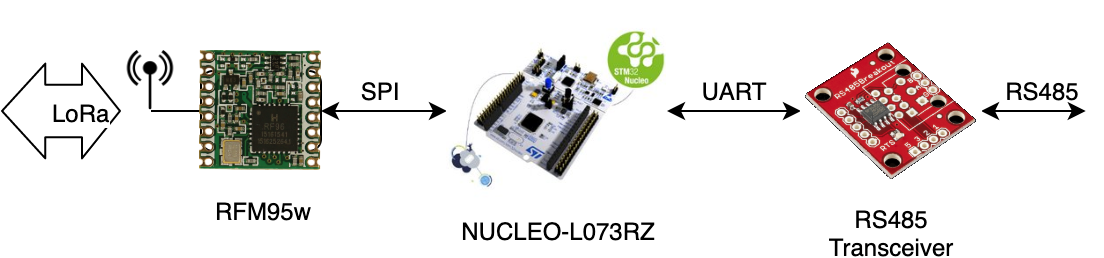
\includegraphics[width=1\textwidth]{LoRaWAN_gw_RS485_blockDiagram_2}
    \caption{Gateway block diagram, RFM95w \cite{RFM95w}, RS485 transceiver \cite{rs485tr}, NUCLEO-L073RZ \cite{nucleoST}}
    \label{fig:gatewayBlockDiagram}
\end{figure}

% The NUCLEO-L073RZ development board with STM32L073RZ microcontroller is suitable for the development purposes because of its parameters, Tab. \ref{tab:mcuFeatures}, price and available documentation.
%It is  was used for the prototype, because it has all required parameters, it is cheap, powerful enough and easily prototypable.
% The price of the devlopment board is \$13 USD\cite{nucleoST}.
% LoRa transceiver board RFM95w with SX1276 chip integrated into Dragino LoRa Shield has the same pinout as the NUCLEO-L073RZ development board. RS485 transceiver as an RS485/UART interface enables communication with Control Panel.

%RS485 transceiver SparkFun Breakout is used for the communication with the Control Panel. It converts interfaces UART to RS485, Fig. \ref{fig:gatewayBlockDiagram}.


% \begin{table}[h]
% \centering
% \footnotesize
% \caption{The STM32L073RZ features \cite{nucleoST}}
% \begin{tabular}{|l|p{3.5cm}|}
% \hline
% Microcontroller architecture & ARM Cortex-M0+ 32-bit RISC \\ \hline
% Internal flash memory & 192 KB \\ \hline
% Internal SRAM memory & 20 kB \\ \hline
% Internal EEPROM memory & 6 kB \\ \hline
% CPU frequency & up to 32 MHz \\ \hline
% Interfaces & 2X SPI, 3x I2C, 4x UART, LIN \\ \hline
% \end{tabular}
% \label{tab:mcuFeatures}
% \end{table}

% \section{Výběr komponent}
% \subsection{Microcontroller}
% Pro toto zařízení je zvolen mikrocontroller STM32L073RZ se zaměřením na nízkou spotřebu, jelikož je levný, má dostačující vlastnosti a je dostupný ve formě vývojového kitu NUCLEO-L073RZ který byl použit pro  vývoj zařízení. Mezi hlavní vlastnosti patří \cite{nucleoST}:
% \begin{itemize}    
%     \item {Architektura ARM Cortex-M0+ 32-bit RISC}
%     \item{Interní Flash paměť 192 KB}
%     \item{Interní SRAM paměť 20 KB}
%     \item{Interní EEPROM paměť 6 KB}
%     \item {Až 32 MHz CPU}
%     \item {2X SPI, 3x I2C, 4x USART, LIN, ADC}
% \end{itemize}

% Pořizovací cena kitu přímo na stránce výrobce www.st.com je \$13 \cite{nucleoST} \cite{nucleoMbed}.
% \begin{figure}[!h]
%     \centering
%     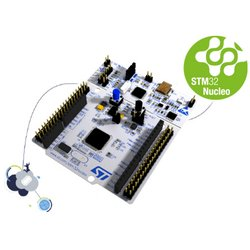
\includegraphics[width=0.4\textwidth]{Nucleo64}
%     \caption{Vývojový kit NUCLEO-L073RZ \cite{nucleoST}}
%     \label{fig:02}
% \end{figure}

% \subsection{LoRa transceiver}
% Lora transceiver čip doposud vyrábí pouze Semtech, pro použití v Evropském pásmu je určen typ SX1276.
% V tomto návrhu je použita deska RFM95w od firmy HopeRF s integrovaným čipem SX1276 \cite{RFM95w}.
% Pro vývoj zařízení byl využit tento transciever v tzv. Dragino LoRa Shield \cite{draginoWiki}, který má stejně jako použitý vývojový kit, pinout kompatibilní s Arduino UNO. Pořizovací cena samotného transceiveru RFM95w je okolo \$7, cena Dragino Shieldu se pohybuje okolo \$22 na ebay.

% \begin{figure}[!h]
%     \centering
%     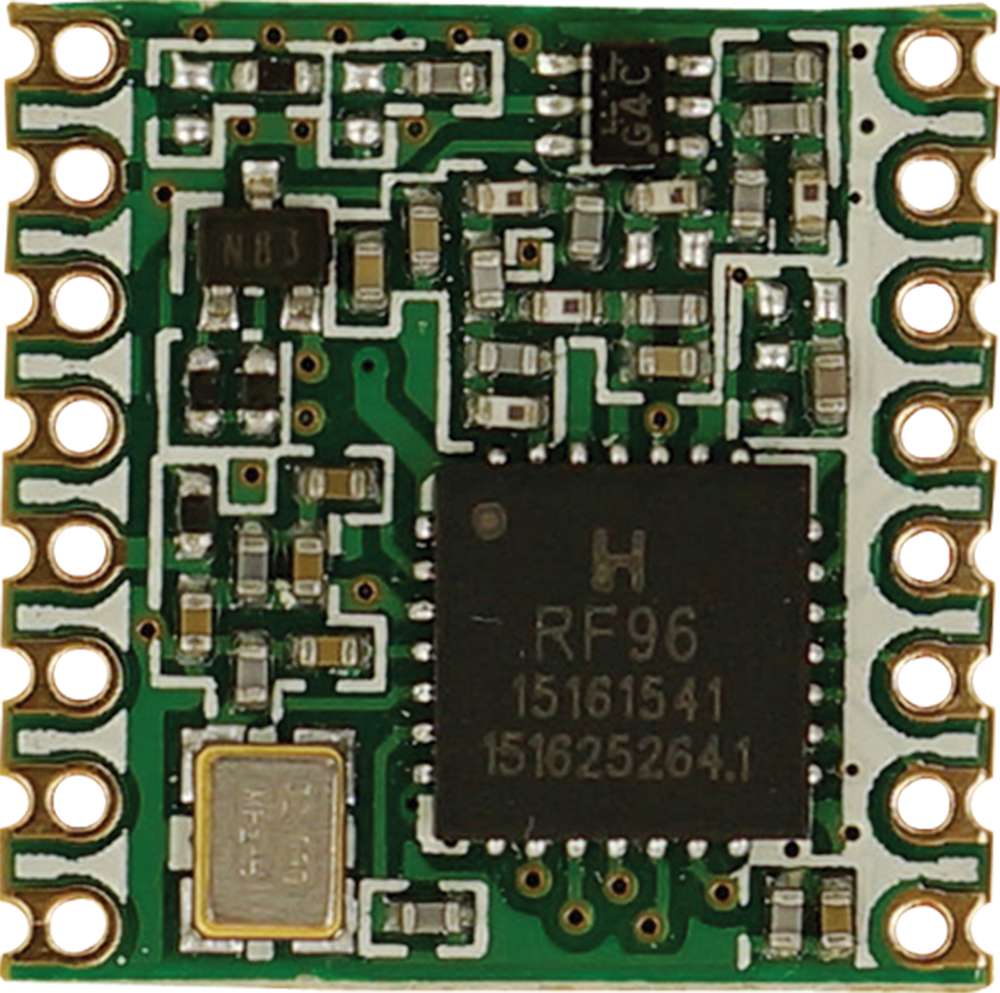
\includegraphics[width=0.2\textwidth]{RFM95w}
%     \caption{LoRa transceiver RFM95w \cite{RFM95w}}
%     \label{fig:02}
% \end{figure}

% \subsection{RS485 transceiver}
% SparkFun Transceiver Breakout - RS485 převádí rozhranní UART na RS485, pří vstupním napětí 3.3 V. A je dostupný za cenu okolo \$10 \cite{rs485tr}.

% \begin{figure}[!h]
%     \centering
%     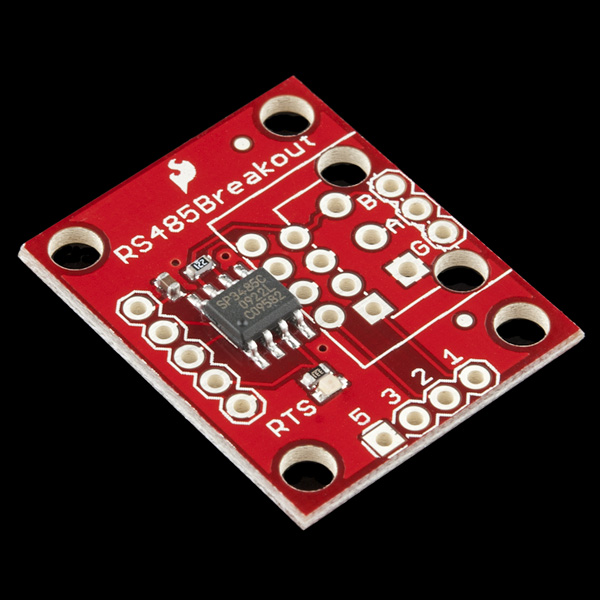
\includegraphics[width=0.4\textwidth]{rs485transceiver}
%     \caption{RS485 transceiver \cite{rs485tr}}
%     \label{fig:rs485transceiver}
% \end{figure}



%%%%%%%%%%%%%%%%%%%%%%%%%%%%%%%%%%%%%%%%%%%%%%%%%%%%%%%%%%%%%%%%%%%%%%%%%%
% \section{Implementace komunkičního protokolu v síti IMA\_RS485 pro komunikaci s control panelem}
% V tomto projektu je komunikace protokolu IMA\_RS485 naprogramována v souborech rs485\_protocol.h a rs485\_protocol.c. 
% Jedná se o kolizní protokol v síti, kde je připojen jedno zařízení typu master, a jeden nebo více zařízení v typu slave.

% \begin{table}[!h]
%     \centering
%     \begin{tabular}{ |c|c| }
%      \hline

%      Baud rate              & 9600           \\ \hline
%      Data bits              & 8                 \\ \hline
%      Parity                 & none              \\ \hline
%      Stop bits              & 1                 \\ \hline

%     \end{tabular}
%     \caption{Fyzické vlastnosti IMA\_RS485 sítě}
%     \label{table:3}
% \end{table}

% \newpage
% \subsection{Syntaxe příkazů}
% Komunikace v síti probíhá formou příkazů, které mají specifikovanou syntaxi v tabulce \ref{table:syntaxePrikazu}.

% \begin{table}[!h]
%     \centering
% \begin{tabular}{ |c|| p{1.5cm} | p{1.5cm} | p{1cm} | p{1cm} | p{1cm} | p{1cm} | }
%  \hline
%  popis      & adresa příjemce & adresa odesílatele & typ příkazu & délka dat & data & crc\\ \hline
%  počet bytů & 1               & 1   & 1     & 2     & délka dat     & 1 \\ 
%  \hline
% \end{tabular}
%     \caption{Syntaxe příkazu pro komunikaci v síti IMA\_RS485}
%     \label{table:syntaxePrikazu}
% \end{table}

% Typy příkazu jsou zadefinované konstanty s předponou CKP\_CMD\_ v souboru ./Inc/rs485\_protocol.h.
% Příkazy odeslané zařízením typu master obsahují navíc synchronizační byte na začátku 0xAA.
% CRC je pro kontrolu XOR přes všechny předchozí byty v celém příkazu kromě synchronizačního bytu.

% \subsection{Adresace zařízení v síti}
% Každé zařízení na této sběrnici má svoji adresu, která mu je nastavena externě. Zařízení typu master má adresu  0xFF, adresa pro všechny (broadcast) je 0x00 a zařízení v této sítí můžou mít adresu libovolnou (krom těchto dvou) nesmí zde však být připojena 2 zařízení s nastavenou stejnou adresou.

% \subsection{Statusy}
% Zařízení typu slave má dva možné statusy v síti IMA\_RS485, offline a online. Zařízení typu slave má povoleno odesílat příkaz "průchod" pouze má-li status online.  
% Zařízení typu slave odesílá příkaz obsahující informaci o jeho statusu periodicky s typem příkazu 0x10 a jedním bytem dat označujícím status. 
% Pro status online je tento byte 0x00 a pro status offline 0xEE. 
% Tento příkaz je odesílán s intervalem 10 s, pokud zařízení má status offline a s intervalem 30 s, pokud má zařízení status online.
% Status zařízení mění pouze zařízení typu master odesláním příkazu s typem 0x41 pro přepnutí na status online a 0x42 pro přepnutí na status offline.
% Zařízení typu slave svůj status přepne samo pouze v případě, že má status online a zařízení typu master přestane odpovídat na příkaz průchod, jak je popsáno v sekci \ref{sec:Odesílání dat z koncových zařízení}.
% Je-li zařízení spuštěno, je ve stavu offline a jelikož nemá povoleno odesílat příkaz "průchod", přijatá data z koncových zařízení jsou zahazována. 
% Zařízení typu slave pouze odpovídá na příkazy od zařízení typu master a čeká na příkaz od zařízení typu master k přepnutí na status online.


% \subsection{Přidávání LoRaWAN zařízení do systému}
% Pokud zařízení typu master přijme příkaz od zařízení typu slave oznamující že je ve stavu offline, nejprve tomuto zařízení pošle seznam LoRaWAN adres všech známých koncových zařízení a následně toto zařízení přepne do stavu online.
% Přijímání seznamu adres je realizováno sekvencí příkazů typu 0x8F. 

% Níže v tabulce \ref{table:2} je příklad sekvence příkazů odesílaných mezi zařízením typu masterem a zařízením typu slavem během předávání seznamu LoRaWAN device address koncových zařízení, kde zařízení typu slave má adresu 0x10 a zařízení typu master standardně 0xFF. Jak již bylo řečeno, příkazy od zařízení typu master lze jednoduše odlišit tím, že vždy začínají bytem 0xAA.


% \begin{table}[!h]
%     \begin{tabular}{ |l|p{10cm}| }
%     \hline
%     příkaz      &  data    \\ \hline \hline
%     master: start      &  AA 10 FF 8F 02 00 00 00 62    \\ \hline
%     slave: ACK        &  FF 10 06 02 00 8F 00 64    \\ \hline
%     master: data     &  AA 10 FF 8F 21 00 01 B1 C4 12 00 00 00 00 00 B2 C4 12 00 00 00 00 00 B3 C4 12 00 00 00 00 00 B4 C4 12 00 00 00 00 00 44 \\ \hline
%     slave: ACK      &  FF 10 06 02 00 8F 01 65   \\ \hline
%     master: data     &  AA 10 FF 8F 19 00 02 B5 C4 12 00 00 00 00 00 B6 C4 12 00 00 00 00 00 F6 1F 01 26 00 00 00 00 B6 \\ \hline
%     slave: ACK      &   FF 10 06 02 00 8F 02 66   \\ \hline
%     master: konec   &   AA 10 FF 8F 04 00 03 FF 2A 57 E5   \\ \hline
%     slave: ACK      &   FF 10 06 02 00 8F 03 67  \\ \hline
%     \end{tabular}
%     \caption{Příklad sekvence příkazů odesílaných mezi zařízením typu master a zařízením typu slave během předávání seznamu LoRaWAN device address koncových zařízení}
%     \label{table:2}
% \end{table}

% LoraWAN protokol používá 4-bytové adresy koncových zařízení.
% Adresy předávány touto sekvencí jsou dlouhé 8-bytové. První 4 byty je tedy LoRaWAN device address, pátý byte je typ zařízení a zbylé 3 byty jsou nevyužity, jejich použití je možné v případě změn či rozšiřování vlastností systému. 

% První Byte dat je counter paketu začínající od nuly, který označuje číslo odeslaného paketu v sekvenci. Na každý tento paket v sekvenci zařízení typu slave odpovídá ACK příkaz, který se liší od obyčejného ACK příkazu tím, že v datech paketu navíc obsahuje counter pakety v sekvenci.
% První příkaz této sekvence má délku dat 2 byty, které mají hodnotu 0x00 přičemž první je counter.
% Další příkazy hned za counter bytem obsahují několik osmibytových adres, jejichž počet je různý.
% Příkaz ukončující tuto sekvenci příkazů má délku 4 byty, což je tedy counter, 0xFF a 2 byty CRC přes všechny odeslané adresy (nepodstatné, tudíž ho nepoužívám).

% \subsection{Odesílání dat z koncových zařízení} 
% \label{sec:Odesílání dat z koncových zařízení}
% Jak je popsáno v sekci \ref{sec:Implementace IoT do přístupového systému firmy IMA}, tudíž data z koncových zařízení jsou odesílána příkazem "průchod", jehož typ je 0x10 a kapacita na data z koncového zařízení je pouze 6 B. 
% První byte dat označuje typ průchodu, byl zvolen konstantní byte 0xD0. Dále následuje LoRaWAN adresa koncového zařízení od kterého byl paket přijat. Dále následují 4 byty dat ze senzoru, další 2 byty signalizující čas průchodu, což v tomto projektu není použito a tyto dva byty mají vždy hodnotu 0xFF. A nakonec jsou další 2 byty obsahující data ze senzoru.
% Příklad příkazu: FF 1F 10 0D 00 D0 F6 1F 01 29 AD 0A 5A 27 FF FF DE 09 E1.
% Data příkazu jsou níže rozepsána v tabulce \ref{table:prikladprikazpruchod}.

% \begin{table}[!h]
%     \centering
% \begin{tabular}{ | p{1.5cm} | p{3cm} | p{2.5cm} | p{1.3cm} | p{1.3cm} |  }
%  \hline
%  typ průchodu & LoRaWAN device address & data (4B)     & cas   & data (2B) \\ \hline
%  D0           & F6 1F 01 29            &  AD 0A 5A 27  & FF FF & DE 09     \\ 
%  \hline
% \end{tabular}
%     \caption{Příklad dat příkazu "průchod" odeslaného z gatewaye na zarizeni typu master, obsahující data z koncových zařízení}
%     \label{table:prikladprikazpruchod}
% \end{table}

% Zařízení typu master na příkaz "průchod" odpovídá příkazem ACK. Zařízení typu slave na tuto odpověď čeká standardně 3 sekundy, ale tento parametr je nastavitelný. Pokud v tomto timeoutu zařízení typu master neodpoví, zařízení typu slave příkaz "průchod" zopakuje přičemž změní typ příkazu na 0x20. Pokud zařízení typu master ani na třetí opakování neodpoví ACK, zařízení typu slave se přepne do stavu offline a vymaže frontu příkazů "průchod" k odeslání.

% \subsection{Potvrzení}
% Zařízení typu slave odpovídá na každý příkaz od zařízení typu master ACK. Typ příkazu ACK je 0x06 a data příkazu obsahují jeden byte signalizující typ příkazu na který je právě odpovídáno potvrzením.
% Zařízení typu master odpovídá ACK se stejným typem příkazu 0x06, ale s žádnými daty příkazu.

% \subsection{Dotaz na příznaky}
% Zařízení typu master se může zeptat s jak dlouhými adresami zařízení typu slave pracuje s typem příkazu 0x49. Zařízení typu slave na to odpovídá ACK s tím, že v datech příkazu je navíc byte 0x04. Zařízení typu master pak počítá s tím, že zařízení typu slave pracuje se 64-bit adresami (ve skutečnosti ale používá 32-bitové a zbylé 4 byty v příkazu průchod jsou pro data z koncového zařízení).

%%%%%%%%%%%%%%%%%%%%%%%%%%%%%%%%%%%%%%%%%%%%%%%%%%%%%%
\subsubsection{Komunikace přes sériovou linku}
\label{Komunikace přes sériovou linku}
Gateway má implementovanou komunikaci přes sériovou linku, umožňující konfiguraci a log. 
K přípojení lze použít PC s libovolnou aplikací umožňující odesílání a přijímání dat zakódovaných ASCII (American Standard Code for Information Interchange) po
sériové lince s nastavením parametrů dle tabulky \ref{table:usb_term}.

\begin{table}[!h]
    \centering
    \begin{ctucolortab}
    \begin{tabular}{ |c|c| }
     \hline

     Baud rate              & 115200           \\ \hline
     Data bits              & 8                 \\ \hline
     Parity                 & none              \\ \hline
     Stop bits              & 1                 \\ \hline
     Flow control           & none               \\ \hline

    \end{tabular}
    \end{ctucolortab}
    \caption{Parametry sériové linky PC terminálu pro komunikaci s gatewayí}
    \label{table:usb_term}
\end{table}

Při komunikaci jsou data standardně oddělována bytem CR (carriage return) 0x0D, ale je akceptována i sekvence CR LF (Line Feed), tedy 0x0D 0x0A. 

%%%%%%%%%%%%%%%%%%%%%%%%%%%%%%%%%%%%%%%%%%%%%%%%%%%%%
\subsection{Log Gatewaye}
Po připojení ke gatewayi přes sériovou linku dle instrukcí v sekci \nameref{Komunikace přes sériovou linku} je možné kontinuálně snímat a log gatewaye obsahující informace o proběhlých událostech. Je-li gateway v normálním pracovním režimu, loguje informace automaticky přes sériovou linku a komunikace je zde pouze jednosměrná, tedy gateway vysílá a PC přijímá.
Níže je příklad výpisu logu v případě, kdy gateway přjala LoRaWAN paket z koncového zařízení senzorové sítě, zpracovala ho a výslednou informaci odeslala na kontrolní panel přes RS485 síť.

\begin{lstlisting}[style=log]
    ________________________________________________
    Rx -> LoRaWAN, pktCntr: 6
    RSSI: -51, SNR: 9, length: 22

    Message type: Unconfirmed Data Up
    Packet rawData: "40F61F0128C0D62508D970CB071595D115BAC68F6663"
    Device Address: "F61F0128"
    FCnt: 9686
    message (encrypted): "D970CB071595D115BA"
    MHDR: 40; FCtrl: C0; FPort: 08; MIC: "C68F6663"
    adaptive data rate: true; ack: false
    message HEX (decrypted): "013566779600FFFFAF"

    Sensor type: RHF1S001
    temperature: 23.30 C, humidity: 52 %
    period: 300 s, RSSI: -51 dBm, SNR: 9 dB, battery voltage: 3.2 V
    Tx -> RS-485: "FF1F100D00D0F61F01281A0934CDFFFF09202E"
    ________________________________________________
    Rx -> RS-485: "AA1FFF060000E6"
    ACK
\end{lstlisting}

Nejprve jsou vypsány data týkající se LoRaWAN protokolu, zašifrovaný i dešifrovaný payload koncového zařízení, typ zařízení a výsledné hodnoty dekódované z payloadu.


%%%%%%%%%%%%%%%%%%%%%%%%%%
\subsection{Konfigurace gatewaye}
\label{Konfigurace gatewaye}
Konfigurace gatewaye se provádí obousměrnou komunikací po sériové lince s připojením dle instrukcí v sekci \nameref{Komunikace přes sériovou linku}.
Po spuštění je gateway v normálním pracovním režimu, přeposílá tedy packety ze senzorové sítě přes RS485 síť na kontrolní panel a informace loguje přes sériovou linku.
Po vstoupení do stavu konfigurace je pozastavena činnost gatewaye, komunikace s koncovými zařízeními LoRaWAN síťě a komunikace s kontrolním panelem v síti RS485 nejsou aktivní.
Do režimu konfigurace je vstoupeno odesláním "config", následuje vypsání současného stavu konfigurace a následně uživatel postupuje zadáním čísla pro výběr možnosti z menu či konkrétního parametru dle vyzvání. Z konfigurace je možné vystoupit kdykoliv bez uložení změn příkazem "quit". 
Procházení jednotlivými menu je navrženo jedodušše tak, aby uživatel nepotřeboval dokumentaci a aby zde vždy bylo uvedeno dost informací pro srozumitelnost.
Níže je zobrazen příklad výpisu po vstupu do konfigurace obsahující informaci o aktuální konfiguraci a hlavní konfigurační menu.

\begin{lstlisting}[style=log]

    _________________Entering configuration setup________________
    
    System configuration:
    
    *** LoRa channel: 
    channel: 0 (868.1 Mhz)
    SF7
    
    *** RS485 channel: 
    my address: 10
    master address: FF
    timeout: 3 s
    
    *** LoRaWAN keys: 
    NwSKey:  FD 90 0D 8C 70 9F 19 24 18 EC FD D4 28 0C AC 47
    AppSKey:  68 9F D0 AC 7A 0F 95 58 B1 19 A0 16 17 F4 16 33
    
    
    Config menu:
    1 -> Config LoRa channel
    2 -> Config RS485 channel
    3 -> Config LoRaWAN protocol
    4 -> Print all LoRaWAN devices
    5 -> Erase all LoRaWAN devices
    6 -> Restore to default configuration
    7 -> Exit without save
    8 -> Save and exit

\end{lstlisting}
    

Jsou zde tedy tři sekce konfigurace, LoRa kanál, RS485 kanál a parametry LoRaWAN protoklu.
Dále jsou zde další možnosti hlavně pro diagnostické účely, a to možnost ručně přidat LoRaWAN koncové zařízení a vymazání všech koncových zařízení, ačkoliv je to obvykle prováděno ze serveru řízení přístupu, a navrácení stavu gatewaye do defaultního stavu. Dále jsou zde možnosti vystoupení z menu s či bez uložení změn, tedy zapsání nově nakonfigurovaných parametrů do non-volatile paměti.

Při procházení jednou ze tří možných konfigurací je vždy pro každý parametr vypsáno jaká data mají být uživatelem zadána v jakém tvaru a zároveň současnou hodnotu měněného parametru. Zadaná data uživatelem jsou vždy zkontrolována zda splňují požadovaný tvar. Pokud ne, uživatel je o tom informován a vván k dalšímu pokusu.
Pokud uživatel některý parametr nehodlá měnit, přeskočí ho odesláním ASCII znaku LF (0x0D) u většiny terminálových aplikací stačí pouze stisknout na klávesnici Enter.
Po provedení některé konfigurace následuje vždy návrat zpět do hlavního menu. Pro uložení nové konfigurace je potřeba v menu vybrat "Save and exit", gateway pak následně vypíše které parametry byly změněny a provede restart. Pokud je vybráno "Exit without save", gateway se pouze restartuje.


\subsubsection{Konfigurace LoRa kanálu}
Položka v menu pod názvem "Config LoRa channel" zahrnuje nastavení SF, tedy přenosovou rychlost a frekvenční kanál. Níže je příklad konfigurace.

\begin{lstlisting}[style=log]
    LoRa channel configuration:
    Enter SF number (7-12)
    (current: 7)
    8
    SF8 set.

    Enter LoRa channel number (0-7)
    ch0 is 868.1 Mhz
    ch1 is 868.3 Mhz
    ch2 is 868.5 Mhz
    ch3 is 867.1 Mhz
    ch4 is 867.3 Mhz
    ch5 is 867.5 Mhz
    ch6 is 867.7 Mhz
    ch7 is 869.0 Mhz
    (current: 0)
    1
    channel 1 set.
\end{lstlisting}

\subsubsection{Konfigurace RS485 kanálu}
Položka v menu pod názvem "Config RS485 channel" zahrnuje nastavení adresy gatewaye, tedy tohoto zařízení, adresy kontrolního panelu a timeout, což je doba čekání na potvrzení od kontrolního panelu po odeslání příkazu "průchod". Níže je příklad konfigurace.

\begin{lstlisting}[style=log]
    RS485 channel configuration:
    Enter address of this device, FF and 00 are reserved.
    (current: 10)
    11
    Address of this device is set to: 11

    Enter master address: 
    (current: FF)
    FE
    Master address is set to: FE

    Enter timeout (seconds)
    (current: 3)
    5
    timeout set to: 5 s
\end{lstlisting}


\subsubsection{Konfigurace LoRaWAN protokolu}
Položka v menu pod názvem "Config LoRaWAN protocol" zahrnuje nastavení šifrovacích klíčů NwkSKey a AppSKey. Níže je příklad konfigurace.

\begin{lstlisting}[style=log]    
    LoRaWAN protocol configuration:
    Enter NwkSKey (16 bytes in HEX)
    (current:  FD 90 0D 8C 70 9F 19 24 18 EC FD D4 28 0C AC 47)
    11111111222222223333333344444444
    NwSKey set to: 11 11 11 11 22 22 22 22 33 33 33 33 44 44 44 44

    Enter AppSKey (16 bytes in HEX)
    (current:  68 9F D0 AC 7A 0F 95 58 B1 19 A0 16 17 F4 16 33)
    11111111222222223333333344444444
    AppSKey set to: 11 11 11 11 22 22 22 22 33 33 33 33 44 44 44 44
\end{lstlisting}


\subsubsection{Print all LoRaWAN devices}
Vypíše všechna LoRaWAN zařízení uložená v paměti. Níže je příklad.


\begin{lstlisting}[style=log]    
    number.......................0:
    Device Address:  B1 C4 12 00
    Device Type: RH1S001
    number.......................1:
    Device Address:  B2 C4 12 00
    Device Type: RH1S001
    number.......................2:
    Device Address:  B3 C4 12 00
    Device Type: RH1S001
    number.......................3:
    Device Address:  B4 C4 12 00
    Device Type: IMA_tempPress
    number.......................4:
    Device Address:  B5 C4 12 00
    Device Type: IMA_tempPress
\end{lstlisting}



\subsubsection{Restore default configuration}
Po zvolení této možnosti je načtena defaultní konfigurace systému, která obsahuje hodnoty viz tabulka \ref{table:5}. Tyto defaultní hodnoty jsou nastaveny v programu a slouží především pro testovací účely.

\begin{table}[!h]
    \centering
    \begin{ctucolortab}
    \begin{tabular}{ |l|l| }
     \hline

     popis              & hodnota         \\ \hline \hline
     RS485 myAddr       & 0x10            \\ \hline
     RS485 MasterAddr   & 0xFF            \\ \hline
     RS485 timeout      & 3               \\ \hline
     LoRa SF            & SF7             \\ \hline
     LoRa channel       & 0 (868.1 Mhz)   \\ \hline
     NwSKey             & FD 90 0D 8C 70 9F 19 24 18 EC FD D4 28 0C AC 47  \\ \hline
     AppSKey            & 68 9F D0 AC 7A 0F 95 58 B1 19 A0 16 17 F4 16 33  \\ \hline

    \end{tabular}
\end{ctucolortab}
    \caption{Defaultní konfigurace systému}
    \label{table:5}
\end{table}



%%%%%%%%%%%%%%%%%%%%%%%%%%%%%%%%%%%%%%%%%%%%%%%%%%%%%%
\subsection{Podpora koncových zařízení}
Jak již bylo zmíněno v sekci \label{Implementace WSN do přístupového systému}, z důvodu datového omezení protokolu sítě RS485 jsou LoRaWAN packety koncových zařízení dekódovány v gatewayi a z dat payloadu vypočítány konečné hodnoty dle dokumentace daného LoRaWAN zařízení a přes síť RS485 na kontrolní panel jsou odeslány pouze vybraná data. Gateway má pro každé koncové zařízení uloženou 4 byty dlouhou adresu a 1 byte typ zařízení.
Momentálně jsou podporovány dva typy koncových zařízení, dle potřeby je možné rozšířit FW gatewaye o další typy koncových zařízení. Tabulka \ref{table:TypyKoncZarizeni} ukazuje hodnotu bytu označující typ koncového zařízení odpovídající konkrétním typům koncových zařízení.

\begin{table}[!h]
    \centering
    \begin{ctucolortab}
    \begin{tabular}{ |l|l| }
     \hline

     Typ zařízení       & Hodnota         \\ \hline \hline
     RHF1S001           & 0x00            \\ \hline
     IMA\_tempPress     & 0x01            \\ \hline
     
    \end{tabular}
    \end{ctucolortab}
    \caption{Typy koncových zařízení}
    \label{table:TypyKoncZarizeni}
\end{table}

% \subsection{Zpracování dat jednotlivých typů koncových zařízení}
Níže je popsáno pro jednotlivá podporovaná koncová zařízení jak jsou data uložena v datové struktuře, jak jsou data z této struktury zpracována a zobrazena a nakonec jak vybraná data jsou zapsána do výsledného bufferu o délce 6 B, který je odeslán přes síť RS485 příkazem "průchod".


\subsubsection{RHF1S001}
Senzor od firmy RisingHF měřící teplotu a vlhkost \cite{RHF1S001 pdf}.

\begin{lstlisting}[style=CStyle]
    /* RHF1S001 data structure */   
    typedef struct {
        int16_t temperature;
        uint8_t humidity;
        uint16_t period;
        int8_t rssi;
        int8_t snr;
        uint8_t battery;
    } RHF1S001_data_t;

    /* Print the data from the structure */
    printf("temperature: %d.%d C, ", RHF1S001_data.temperature / 100, RHF1S001_data.temperature % 100);
    printf("humidity: %d %%\n", RHF1S001_data.humidity);
    printf("period: %d s, ", (int)RHF1S001_data.period);
    printf("RSSI: %d dBm, ", RHF1S001_data.rssi);
    printf("SNR: %d dB, ", RHF1S001_data.snr);
    printf("battery voltage: %d.%d V\r\n", RHF1S001_data.battery/10, RHF1S001_data.battery % 10);

    /* Put the data into 6 B long buffer, to be transmitted to the control panel */
    buffer[0] = RHF1S001_data.temperature & 0xFF;
    buffer[1] = RHF1S001_data.temperature >> 8;
    buffer[2] = RHF1S001_data.humidity;
    buffer[3] = RHF1S001_data.rssi;
    buffer[4] = RHF1S001_data.snr;
    buffer[5] = RHF1S001_data.battery;
\end{lstlisting}


\subsubsection{IMA\_tempPress}
Senzor vytvořený ve firmě IMA, měřící teplotu a tlak.

\begin{lstlisting}[style=CStyle]
    /* IMA_tempPress data structure */   
    typedef struct {
        int16_t temperature;
        uint16_t pressure;
        int8_t rssi;
        int8_t snr;
    } IMA_tempPress_data_t;
    
    /* print the data from the structure */
    printf("temperature: %d.%d C, ", IMA_tempPress_data.temperature / 100, IMA_tempPress_data.temperature % 100);
    printf("pressure: %d.%d Pa\r\n", IMA_tempPress_data.pressure/10, IMA_tempPress_data.pressure % 10);
    printf("RSSI: %d dBm, SNR: %d dB\r\n", IMA_tempPress_data.rssi, IMA_tempPress_data.snr);

    /* Put the data into 6B long buffer, that is transmitted to the K4 server */
    buffer[0] = IMA_tempPress_data.temperature & 0xFF;
    buffer[1] = IMA_tempPress_data.temperature >> 8;
    buffer[2] = IMA_tempPress_data.pressure & 0xFF;
    buffer[3] = IMA_tempPress_data.pressure >> 8;
    buffer[4] = IMA_tempPress_data.rssi;
    buffer[5] = IMA_tempPress_data.snr;
\end{lstlisting}


%%%%%%%%%%%%%%%%%%%%%%%%%%%%%%%%%%%%%%%%%%%%%%%%%%%%%%
\section{Přidávání koncových zařízení ze serveru řízení přístupu}
Přidávání koncových zařízení senzorové sítě se provádí z uživatelského rozhranní serveru řízení přístupu stejně jako přidávání platných RFID karet, s délkou UID 8 B.
Adresa koncového zařízení (LoRaWAN device address) je dlouhá 4 B, jeden byte je navíc použit pro typ koncového zařízení, zbylé 3 byty jsou nuly.
Jelikož typ zařízení je uložen v gatewayi i na serveru řízení přístupu. Při odesílání příkazu "průchod" se tedy už typ zařízení neposílá z důvodu omezené velikosti tohoto příkazu.
Na serveru řízení přístupu se UID nastavuje jako dekadické číslo.

Pro případ, kde typ zařízení je 01 a DevAddr AABBCCDD (little endian) výsledné číslo v hexadecimální podobě je 01DDCCBBAA. Následně se překládá do decimalni podoby, výsledné číslo k zadání do uživatelského rozhranní serveru řízení přístupu je tedy 8016149418.



%%%%%%%%%%%%%%%%%%%%%%%%%%%%%%%%%%%%%%%%%%%%%%%%%%%%%%
% \section{Využití non-volatile paměťi gatewaye}
% Konfigurace a adresy s typy všech koncových zařízení v LoRaWAN síti jsou uloženy v non-volatile paměti EEPROM gatewaye o kapacitě 6144 B. 
% Paměť je tedy rozdělená tak, že od adresy 0 až po 6080 je prostor pro ukládání LoRaWAN zařízení a od 6080 až po 6144 je prostor pro ukládání konfigurace gatewaye.

% Každé LoRaWan zařízení v síti má v paměti uložené LoRaWAN device address (4 byty), typ zařízení (1 byte) a další 3 byty jsou rezervovány. 
% Jedno koncové zařízení v paměti tedy zabírá  8 B, takže gateway má kapacitu paměti pro až 760 koncových zařízení.


%%%%%%%%%%%%%%%%%%%%%%%%%%%%%%%%%%%%%%%%%%%%%%%%%%%%%%
% \section{Zapojení}
% LoRa shield \cite{draginoWiki} je nasazen přímo na vývojový kit Nukleo. Kit neobsahuje ISCP konektor, který je součástí pinoutu Arduino UNO a LoRa shield má SPI piny MISO a MOSI přivedeny právě na tento konektor. Musí být tedy propojeny externě viz obrázek \ref{fig:03}. Jumpery na Dragino LoRa shieldu musí také být stejně jako v obrázku.

% \begin{figure}[!h]
%     \centering
%     \includegraphics[width=1\textwidth]{foto01}
%     \caption{foto zapojení}
%     \label{fig:03}
% \end{figure}

% Pro komunikaci s LoRa transceiverem je tedy použito SPI1, pro komunikaci přes USB je použito USART2 a pro komunikaci přes RS485 je použito UART1.

% \begin{table}[h]
%     \centering
%     \begin{tabular}{ |c|c|c| }
%      \hline

%      Periférie          & Název pinu & Pin procesoru           \\ \hline \hline
     
%                         & RX  &   PC1            \\
%     RS485 transceiver   & TX  &   PC0       \\
%                         & RTS  &  PB1      \\     \hline

%                         & CS    &  PB6             \\
%                         & CLK   &  PA5        \\
%    LoRa transceiver     & MISO  &  PA6     \\
%                         & MOSI  &  PA7        \\
%                         & RST   & PC7          \\
%                         & DIO0  & PA10         \\
%                         \hline

%     \end{tabular}
%     \caption{Pinout připojení externích periférií k procesoru}
%     \label{table:3}
% \end{table}

%%%%%%%%%%%%%%%%%%%%%%%%%%%%%%%%%%%%%%%%%%%%%%%%
% \section{Naprogramování}
% K naprogramování MCU byla použita HAL knihovna a inicializační nástroj STM32CubeMX poskytnuté výrobcem, tedy ST Microelectronics.
% Zdrojové soubory programu byly vyvíjeny v textovém editoru VS-Code, ke kompilaci zdrojových souborů byl použit kompilátor arm-none-eabi-gcc a jako pomocný nástroj makefile skript. 

% \subsection{Zdrojové soubory projektu}
% Pro šifrování LoRaWAN paketu byla použita knihovna AES-128, dostupná na githubu \cite{AESlib} a knihovna OpenPANA také dostupná z githubu \cite{CMAClib}.
% Níže je seznam zdrojových souborů.

% \begin{figure}[!h]
%     \dirtree{%
%         .1 Drivers \DTcomment{STM32 Drivers}.
%         .1 Inc\DTcomment{Headers}.
%             .2 aes.h\DTcomment{AES-128 library for LoRaWAN paket encryption}.
%             .2 cmac.h\DTcomment{library for CMAC calculation in LoRaWAN protocol}.
%             .2 LinkedList\_ByteArray.h \DTcomment{Byte array linked list library for stacks}.
%             .2 LoRaWAN\_paket.h\DTcomment{LoRaWAN library for paket data decoding}.
%             .2 stm32l0xx\_hal\_conf.h\DTcomment{HAL initialization of peripherals}.
%             .2 ByteArray.h\DTcomment{Library for Byte array operations}.
%             .2 LoRa.h\DTcomment{Library for interfacing LoRa transceiver}.
%             .2 main.h\DTcomment{Main file}.
%             .2 stm32l0xx\_it.h\DTcomment{HAL initialization of peripherals}.
%             .2 eeprom.h\DTcomment{Library for eeprom operations}.
%             .2 LoRa\_sensors.h\DTcomment{Library for decoding data from payload}.
%             .2 rs485\_protocol.h\DTcomment{Library for RS485 IMA protocol}.
%             .2 usb.h \DTcomment{Library for USB communication and system configuration}.
%         .1 Src\DTcomment{Sources}.
%             .2 aes.c \DTcomment{source file to the aes.h}.
%             .2 aes.c \DTcomment{source file to the cmac.h}.
%             .2 LinkedList\_ByteArray.c \DTcomment{source file to the LinkedList\_ByteArray.h}.
%             .2 LoRaWAN\_paket.c  \DTcomment{source file to the LoRaWAN\_paket.h}.
%             .2 stm32l0xx\_hal\_msp.c \DTcomment{HAL source file}.
%             .2 ByteArray.c  \DTcomment{source file to the ByteArray.h}.
%             .2 LoRa.c \DTcomment{source file to the LoRa.h}.
%             .2 main.c \DTcomment{main source file}.
%             .2 stm32l0xx\_it.c \DTcomment{HAL source file}.
%             .2 eeprom.c \DTcomment{source file to the eeprom.h}.
%             .2 LoRa\_sensors.c \DTcomment{source file to the LoRa\_sensors.h}.
%             .2 rs485\_protocol.c  \DTcomment{source file to the rs485\_protocol.h}.
%             .2 system\_stm32l0xx.c \DTcomment{HAL source file}.
%             .2 usb.h \DTcomment{source file to the usb.h}.
%     }
% \end{figure}


% \subsection{Nahrání programu do MCU}
% Výstupem kompilace je soubor s koncovkou .binary, který je nahrán do MCU. K tomuto nahrání není potřeba žádný speciální SW nebo HW.
% Stačí kit připojit k PC přes USB, v PC se kit zobrazí jako flash disk. Zkompilovaný program s koncovkou .binary stačí překopírovat na toto zařízení. 
% Po dobu kopírování souboru bliká na kitu LED1 červená/zelená. Jakmile kopírování skončí, program na kitu je spuštěn, případně je možné kit resetovat černým tlačítkem reset.
% Pro uvedení Gatewaye do provozu je nutné se připojit k zařízení přes USB a nastavit všechny parametry viz sekce \ref{sec:konfigurace}.  